
Skaliaras - vienas skaičius. \textit{Angl. scalar, scale} \\
Vektorius - skaliarų sąrašas, pavyzdžiui: $\{x; y; z; 40, 50\}$. Vektorius galima pavaizduoti plokštumoje naudojant atkarpą.

\begin{table}[h]
    \begin{tabular}{rll}
        Skaliaras & $a$ \\
        Vektorius & $\{a_1; a_2 \dots a_n\}$\\
        Matrica   & $\begin{bmatrix}
            a_1 & a_2 & \dots & a_n \\
            b_1 & b_2 & \dots & b_n \\
            \dots & \dots & \dots & \dots
        \end{bmatrix}$ \\
        \dots & \dots
    \end{tabular}
    \hspace{40mm}
    \begin{tabular}{rc}
        Ašis & Pavadinimas \\ \hline
        OX & Abscisių ašis \\
        OY & Ordinačių ašis \\
        OZ & Aplikačių ašis
    \end{tabular}
\end{table}
Mes naudojame vektorius, kurie turi: $\{x; y\}$ arba $\{x; y; z\}$. Pavyzdžiui: $\vec{AB}(3;\,4)$.

\begin{wrapfigure}{l}{0.4\textwidth}
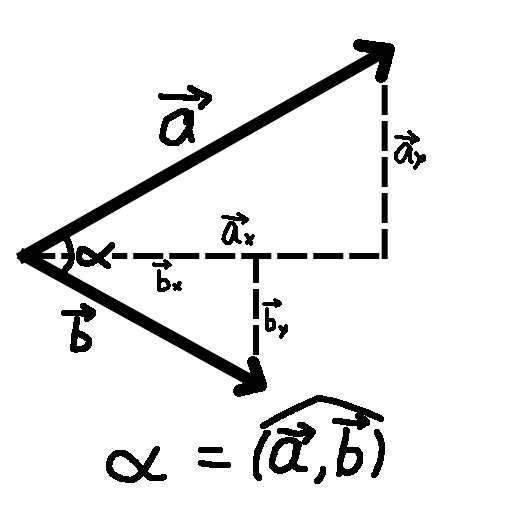
\includegraphics[scale=0.4]{vector_basics.png}
\end{wrapfigure}

\begin{equation}
    \hspace{10mm}
    \begin{aligned}
        \vec{AB} & (x_2 - x_1; y_2 - y_1; z_2 - z_1) \\
        \vec{i} & (1, 0, 0), \vec{j}(0, 1, 0), \vec{k}(0, 0, 1) \\
        \vec{AB} &= (x_2 - x_1) \cdot \vec{i} + (y_2 - y_1) * \vec{j} + (z_2 - z_1) \cdot \vec{k} \\
        |\vec{AB}| &= \sqrt{x^2 + y^2 + z^2} \\
        \vec{AB} + \vec{BC} &= \vec{AC} \ne \vec{CA} \\
        \vec{AB} - \vec{BC} &= -\vec{AC} = \vec{CA} \\
        \vec{a} \cdot n &= \vec{a} + \vec{a} + \dots \}\ n \text{ kartų} \\
        \vec{a} \cdot \vec{b} &= |\vec{a}| \cdot |\vec{b}| \cdot \cos{\widehat{(\vec{a}; \vec{b})}} \\
        \vec{a} \cdot \vec{b} &= \vec{a}_x \cdot \vec{b}_x + \vec{a}_y \cdot \vec{b}_y \\
        \vec{a} \cdot \vec{b} &= \frac{\vec{a} \cdot \vec{b}}{|\vec{a}||\vec{b}|}
    \end{aligned}
\end{equation}

\begin{table}[h]
    \begin{tabular}{rcl}
        Vektoriaus tipas& Pavyzdžiai & Apibrėžimas \\ \hline
        Kolinearieji    & \includegraphics*[scale=0.25]{colinear_vectors.png} & $\vec{a}_x : \vec{b}_y = \vec{a}_x : \vec{b}_x$ \\
        Vienkrypčiai    & \includegraphics*[scale=0.25]{one-way_vectors.png} & $\vec{a} \uparrow \uparrow \vec{b}, \vec{a} \cdot m = \vec{b}, m > 0$  \\
        Priešpriešiniai & \includegraphics*[scale=0.25]{opposite-facing_vectors.png} & $\vec{a} \uparrow \downarrow \vec{b}, \vec{a} \cdot m = \vec{b}, m < 0$ \\
        Statmeni        & \includegraphics*[scale=0.25]{perpendicular_vectors.png} & $\vec{a} \perp \vec{b}, \;\vec{a} \cdot \vec{b} = 0 $ \\
        Lygieji         & \includegraphics*[scale=0.25]{equal_vectors.png} & $\vec{a} = \vec{b}$ \\
        Priešingieji    & \includegraphics*[scale=0.25]{opposite_vectors.png} & $\vec{a} = -\vec{b}$ \\
        Nulinis         & $\vec{AA}$ & $|\vec{a}| = 0$
    \end{tabular}
\end{table}

\clearpage

\subsection{Vektorių sudėtis}
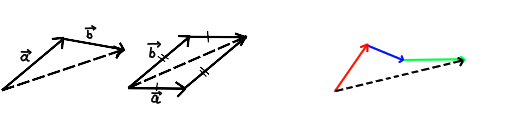
\includegraphics{assets/vector_addition.png}

\subsubsection{Pratimai}

Išreiškite vektorius, kuriuos reikėtų sudėti, kad gautumėte $\vec{AZ}$

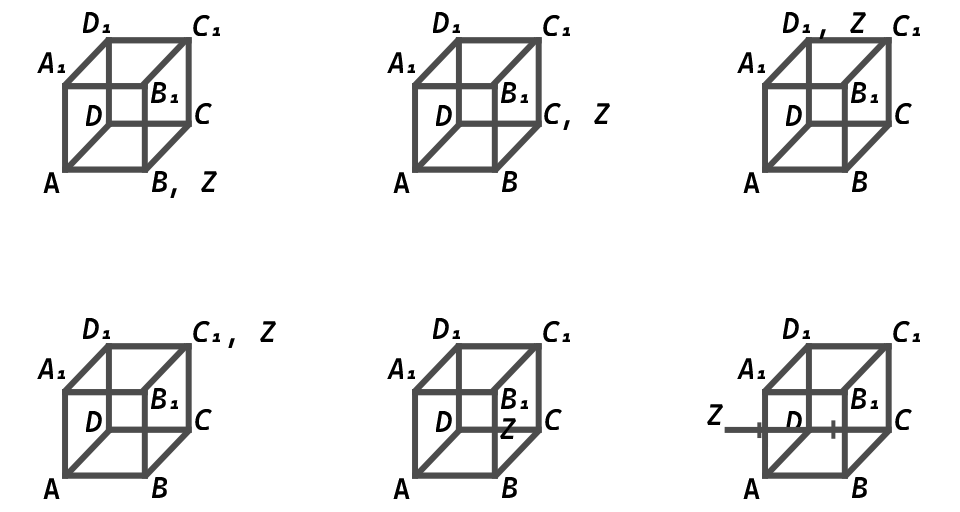
\includegraphics[max width=\textwidth]{assets/vector_exercise.png}
Raskite dydžius, kai A(10; 11), B(7; 7), C(4, 1), D(15, 13): \\
\begin{exercises}
    \item $|\vec{AB}|                           $
    \item $\vec{AB} + \vec{CD}                  $
    \item $\vec{AD} \cdot 2                     $
    \item $\vec{AB} \cdot \vec{CD}              $
    \item $\frac{\vec{AB}}{\vec{CD}}            $
    \item $\cos \widehat{(\vec{AB}, \vec{DC})}  $
\end{exercises}

\subsubsection{Daugiau}

$\vec{a} \ne (\vec{a}_x; \vec{a}_y)$, nes $(a_1, a_2 \dots )$ yra sekos sintaksė.

\clearpage

